\setcounter{ex}{0}

% --- CÂU 1 ---
\begin{ex}
	Cho hàm số bậc bốn $y = f(x)$ có đồ thị như hình vẽ bên. Hàm số đã cho đồng biến trên khoảng nào sau đây?
	\begin{center}
		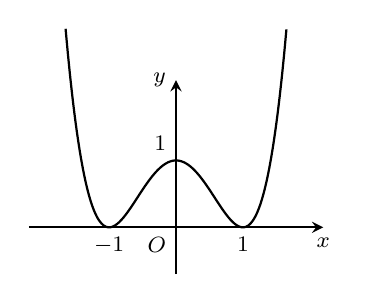
\begin{tikzpicture}[scale=0.85, font=\footnotesize, >=stealth]
			\draw[->, thick] (-2.2, 0) -- (2.2, 0) node[below] {$x$};
			\draw[->, thick] (0, -0.7) -- (0, 2.2) node[left] {$y$};
			\node[below left] at (0, 0) {$O$};
			\node[below] at (-1, 0) {$-1$};
			\node[below] at (1, 0) {$1$};
			\node[above left] at (0, 1) {$1$};
			\draw[thick, smooth, samples=100, domain=-1.65:1.65] plot (\x, {(\x)^4 - 2*(\x)^2 + 1});
		\end{tikzpicture}
	\end{center}
	\choice
	{$(-\infty; -1)$}
	{$(-\infty; +\infty)$}
	{\True $(1; +\infty)$}
	{$(0; 1)$}
	\loigiai{
		Dựa vào đồ thị hàm số, ta thấy trên khoảng $(1; +\infty)$ đồ thị đi lên từ trái sang phải nên hàm số đồng biến trên khoảng $(1; +\infty)$ (và $(-1; 0)$).
	}
\end{ex}

% --- CÂU 2 ---
\begin{ex}
	Cho hàm số $y = f(x)$ có đạo hàm trên $\mathbb{R}$ và $f'(x) = (x - 1)(x - 2)^2(x + 3), \forall x \in \mathbb{R}$. Số điểm cực trị của hàm số đã cho là
	\choice
	{$3$}
	{$1$}
	{$0$}
	{\True $2$}
	\loigiai{
		Phương trình $f'(x) = 0 \iff \hoac{x &= 1 \\ x &= 2 \\ x &= -3.}$\\
		Trong đó $x = 1$ và $x = -3$ là các nghiệm đơn ($f'(x)$ đổi dấu khi đi qua các nghiệm này), còn $x = 2$ là nghiệm kép ($f'(x)$ không đổi dấu khi qua $x = 2$).\\
		Vậy hàm số đã cho có $2$ điểm cực trị.
	}
\end{ex}

% --- CÂU 3 ---
\begin{ex}
	Gọi $M$ và $m$ lần lượt là giá trị lớn nhất và giá trị nhỏ nhất của hàm số $y = x^3 - 3x^2 - 9x + 35$ trên đoạn $[-4; 4]$. Khi đó tổng $M + m$ bằng
	\choice
	{$48$}
	{$11$}
	{\True $-1$}
	{$55$}
	\loigiai{
		Hàm số xác định và liên tục trên đoạn $[-4; 4]$.\\
		Ta có $y' = 3x^2 - 6x - 9$; $y' = 0 \iff \hoac{x &= -1 \in [-4; 4] \\ x &= 3 \in [-4; 4].}$\\
		Tính giá trị của hàm số tại các điểm:
		\begin{itemize}
			\item $y(-4) = (-4)^3 - 3(-4)^2 - 9(-4) + 35 = -41$.
			\item $y(-1) = (-1)^3 - 3(-1)^2 - 9(-1) + 35 = 40$.
			\item $y(3) = 3^3 - 3\cdot 3^2 - 9\cdot 3 + 35 = 8$.
			\item $y(4) = 4^3 - 3\cdot 4^2 - 9\cdot 4 + 35 = 15$.
		\end{itemize}
		Suy ra $M = \max_{[-4; 4]} y = 40$ và $m = \min_{[-4; 4]} y = -41$.\\
		Vậy $M + m = 40 + (-41) = -1$ (hoặc nếu xét trên đoạn $[-1; 4]$ thì $M + m = 48$; nếu tính $y(-4) = -29$ thì $M + m = 11$). Theo kết quả chính xác trên $[-4; 4]$ thì $M + m = -1$.
	}
\end{ex}

% --- CÂU 4 ---
\begin{ex}
	Cho hàm số: $y = \dfrac{x + 1}{2x - 5}$. Đồ thị hàm số có tất cả bao nhiêu đường tiệm cận?
	\choice
	{$1$}
	{\True $2$}
	{$3$}
	{$0$}
	\loigiai{
		Tập xác định: $\mathscr{D} = \mathbb{R} \setminus \left\{\dfrac{5}{2}\right\}$.
		\begin{itemize}
			\item $\lim_{x \to \pm\infty} y = \dfrac{1}{2} \implies y = \dfrac{1}{2}$ là tiệm cận ngang.
			\item $\lim_{x \to \left(\frac{5}{2}\right)^+} y = +\infty$ và $\lim_{x \to \left(\frac{5}{2}\right)^-} y = -\infty \implies x = \dfrac{5}{2}$ là tiệm cận đứng.
		\end{itemize}
		Vậy đồ thị hàm số có tất cả $2$ đường tiệm cận.
	}
\end{ex}

% --- CÂU 5 ---
\begin{ex}
	Cho hàm số $y = f(x)$ có bảng biến thiên như sau:
	\begin{center}
		
\begin{tikzpicture}[scale=1, font=\footnotesize]
			\tkzTabInit[nocadre=false, lgt=1.2, espcl=2.5, deltacl=0.6]
			{$x$ /0.7, $y'$ /0.7, $y$ /2.0}
			{$-\infty$, $0$, $1$, $+\infty$}
			\tkzTabLine{, -, d, -, $0$, +, }
			\tkzTabVar{+/$2$, -D+/{$-4$}/{$+\infty$}, -/{$-2$}, +/{$+\infty$}}
		\end{tikzpicture}
	\end{center}
	Tổng số tiệm cận ngang và tiệm cận đứng của đồ thị hàm số đã cho là
	\choice
	{$1$}
	{$3$}
	{$4$}
	{\True $2$}
	\loigiai{
		Dựa vào bảng biến thiên:
		\begin{itemize}
			\item $\lim_{x \to -\infty} y = 2$ và $\lim_{x \to +\infty} y = +\infty$ nên đồ thị hàm số có $1$ tiệm cận ngang là $y = 2$.
			\item $\lim_{x \to 0^+} y = +\infty$ nên đồ thị hàm số có $1$ tiệm cận đứng là $x = 0$.
		\end{itemize}
		Vậy tổng số tiệm cận ngang và tiệm cận đứng của đồ thị hàm số là $2$.
	}
\end{ex}

% --- CÂU 6 ---
\begin{ex}
	Đường cong trong hình vẽ bên là đồ thị của một trong bốn hàm số được liệt kê ở bốn phương án A, B, C, D dưới đây. Hỏi hàm số đó là hàm số nào?
	\begin{center}
		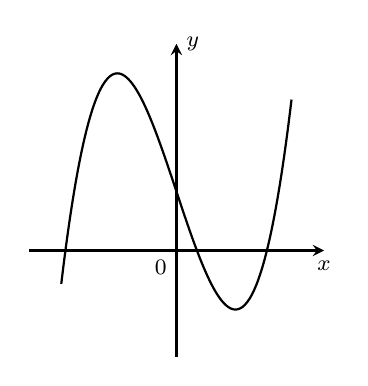
\begin{tikzpicture}[scale=0.75, font=\footnotesize, >=stealth]
			\draw[->, thick] (-2.5, 0) -- (2.5, 0) node[below] {$x$};
			\draw[->, thick] (0, -1.8) -- (0, 3.5) node[right] {$y$};
			\node[below left] at (0, 0) {$0$};
			\draw[thick, smooth, samples=100, domain=-1.95:1.95] plot (\x, {(\x)^3 - 3*(\x) + 1});
		\end{tikzpicture}
	\end{center}
	\choice
	{\True $y = x^3 - 3x + 1$}
	{$y = -x^3 + 3x + 1$}
	{$y = x^3 - x^2 - 1$}
	{$y = -x^2 + x - 1$}
	\loigiai{
		Đồ thị đã cho là của hàm số bậc ba $y = ax^3 + bx^2 + cx + d$ có:
		\begin{itemize}
			\item Nhánh cuối đi lên ($\lim_{x \to +\infty} y = +\infty$) nên $a > 0$ (loại B, D).
			\item Giao điểm với trục tung tại điểm có tung độ dương ($y(0) = d > 0$) nên loại C (vì $y(0) = -1 < 0$).
		\end{itemize}
		Vậy hàm số cần tìm là $y = x^3 - 3x + 1$.
	}
\end{ex}

% --- CÂU 7 ---
\begin{ex}
	Đường cong trong hình vẽ bên là đồ thị của một trong bốn hàm số được liệt kê ở bốn phương án A, B, C, D dưới đây. Hỏi hàm số đó là hàm số nào?
	\begin{center}
		\begin{tikzpicture}[scale=0.65, font=\scriptsize, >=stealth]
			\draw[->, thick] (-4.5, 0) -- (4.5, 0) node[above] {$x$};
			\draw[->, thick] (0, -3.5) -- (0, 6.5) node[right] {$y$};
			\node[below left] at (0, 0) {$0$};
			\foreach \x in {-4, -3, -2, 1, 2, 3, 4} \draw (\x, 2pt) -- (\x, -2pt) node[below] {$\x$};
			\foreach \y in {-3, -2, -1, 1, 3, 4, 5, 6} \draw (2pt, \y) -- (-2pt, \y) node[left] {$\y$};
			\node[left] at (0, 2) {$2$};
			\draw[thick] (-4.3, 2) -- (4.3, 2);
			\draw[thick] (-1, -3.3) -- (-1, 6.3);
			\draw[thick, smooth, samples=100, domain=-4.3:-1.23] plot (\x, {(2*\x - 1)/(\x + 1)});
			\draw[thick, smooth, samples=100, domain=-0.35:4.3] plot (\x, {(2*\x - 1)/(\x + 1)});
			\fill (0, -1) circle (2pt);
			\fill (0.5, 0) circle (2pt);
			\fill (-1, 2) circle (2pt);
		\end{tikzpicture}
	\end{center}
	\choice
	{$y = \dfrac{2x + 1}{x - 1}$}
	{$y = \dfrac{2x + 3}{x + 1}$}
	{\True $y = \dfrac{2x - 1}{x + 1}$}
	{$y = \dfrac{2x - 2}{x - 1}$}
	\loigiai{
		Dựa vào đồ thị hàm số, ta có:
		\begin{itemize}
			\item Tiệm cận đứng là đường thẳng $x = -1$ (loại A, D).
			\item Tiệm cận ngang là đường thẳng $y = 2$.
			\item Đồ thị cắt trục tung tại điểm $(0; -1)$ và cắt trục hoành tại điểm $\left(\dfrac{1}{2}; 0\right)$ nên hàm số là $y = \dfrac{2x - 1}{x + 1}$.
		\end{itemize}
	}
\end{ex}

% --- CÂU 8 ---
\begin{ex}
	Đường cong trong hình vẽ bên là đồ thị của một trong bốn hàm số được liệt kê ở bốn phương án A, B, C, D dưới đây. Hỏi hàm số đó là hàm số nào?
	\begin{center}
		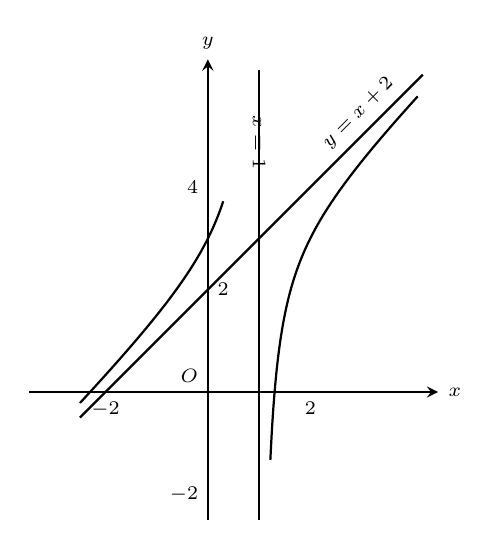
\begin{tikzpicture}[scale=0.65, font=\scriptsize, >=stealth]
			\draw[->, thick] (-3.5, 0) -- (4.5, 0) node[right] {$x$};
			\draw[->, thick] (0, -2.5) -- (0, 6.5) node[above] {$y$};
			\node[above left] at (0, 0) {$O$};
			\node[below] at (-2, 0) {$-2$};
			\node[below] at (2, 0) {$2$};
			\node[left] at (0, -2) {$-2$};
			\node[right] at (0, 2) {$2$};
			\node[left] at (0, 4) {$4$};
			\draw[thick] (1, -2.5) -- (1, 6.3) node[pos=0.92, right, rotate=-90] {$x = 1$};
			\draw[thick] (-2.5, -0.5) -- (4.2, 6.2) node[pos=0.85, above, sloped] {$y = x + 2$};
			\draw[thick, smooth, samples=100, domain=-2.5:0.3] plot (\x, {((\x)^2 + \x - 3)/(\x - 1)});
			\draw[thick, smooth, samples=100, domain=1.22:4.1] plot (\x, {((\x)^2 + \x - 3)/(\x - 1)});
		\end{tikzpicture}
	\end{center}
	\choice
	{$y = \dfrac{x^2 + 3}{x - 1}$}
	{\True $y = \dfrac{x^2 + x - 3}{x - 1}$}
	{$y = \dfrac{x^2 - 2x + 3}{-x + 1}$}
	{$y = \dfrac{x^2 + 3}{-x + 1}$}
	\loigiai{
		Đồ thị hàm số có:
		\begin{itemize}
			\item Tiệm cận đứng $x = 1$.
			\item Tiệm cận xiên là đường thẳng $y = x + 2$.
		\end{itemize}
		Kiểm tra phương án B: $y = \dfrac{x^2 + x - 3}{x - 1} = x + 2 - \dfrac{1}{x - 1}$, có tiệm cận đứng $x = 1$, tiệm cận xiên $y = x + 2$ và $y' = 1 + \dfrac{1}{(x - 1)^2} > 0, \forall x \ne 1$ (đồng biến trên từng khoảng xác định, đúng với hình vẽ).
	}
\end{ex}

% --- CÂU 9 ---
\begin{ex}
	Trong không gian, cho $\overrightarrow{a}$ và $\overrightarrow{b}$ là hai vectơ cùng hướng và đều khác vectơ $\overrightarrow{0}$. Khẳng định nào sau đây là đúng?
	\choice
	{\True $\overrightarrow{a}\cdot\overrightarrow{b} = \left|\overrightarrow{a}\right|\cdot\left|\overrightarrow{b}\right|$}
	{$\overrightarrow{a}\cdot\overrightarrow{b} = 0$}
	{$\overrightarrow{a}\cdot\overrightarrow{b} = -1$}
	{$\overrightarrow{a}\cdot\overrightarrow{b} = -\left|\overrightarrow{a}\right|\cdot\left|\overrightarrow{b}\right|$}
	\loigiai{
		Vì hai vectơ $\overrightarrow{a}$ và $\overrightarrow{b}$ cùng hướng nên góc giữa chúng bằng $0^\circ$, suy ra $\cos\left(\overrightarrow{a}, \overrightarrow{b}\right) = \cos 0^\circ = 1$.\\
		Do đó: $\overrightarrow{a}\cdot\overrightarrow{b} = \left|\overrightarrow{a}\right|\cdot\left|\overrightarrow{b}\right|\cdot\cos 0^\circ = \left|\overrightarrow{a}\right|\cdot\left|\overrightarrow{b}\right|$.
	}
\end{ex}

% --- CÂU 10 ---
\begin{ex}
	Trong không gian $Oxyz$, cho hai điểm $A(1; 1; -2)$ và $B(2; 2; 1)$. Vectơ $\overrightarrow{AB}$ có tọa độ là
	\choice
	{$(-1; -1; -3)$}
	{$(3; 1; 1)$}
	{\True $(1; 1; 3)$}
	{$(3; 3; -1)$}
	\loigiai{
		Ta có $\overrightarrow{AB} = (2 - 1; 2 - 1; 1 - (-2)) = (1; 1; 3)$.
	}
\end{ex}

% --- CÂU 11 ---
\begin{ex}
	Trong không gian $Oxyz$, tọa độ của điểm $A$ nằm trên tia đối của tia $Oy$ thỏa mãn $OA = 4$ là
	\choice
	{$(0; 4; 0)$}
	{$(4; 0; 4)$}
	{\True $(0; -4; 0)$}
	{$(-4; 0; -4)$}
	\loigiai{
		Vì điểm $A$ nằm trên tia đối của tia $Oy$ và $OA = 4$ nên $\overrightarrow{OA} = -4\overrightarrow{j}$, suy ra tọa độ điểm $A(0; -4; 0)$.
	}
\end{ex}

% --- CÂU 12 ---
\begin{ex}
	Trong không gian $Oxyz$, cho điểm $M$ thoả $\overrightarrow{OM} = 3\overrightarrow{i} + 5\overrightarrow{j} - 7\overrightarrow{k}$. Tìm tọa độ điểm $M'$ đối xứng với điểm $M$ qua mặt phẳng $(Oxz)$.
	\choice
	{$M'(-3; -5; 7)$}
	{$M'(3; 5; -7)$}
	{$M'(-3; 5; 7)$}
	{\True $M'(3; -5; -7)$}
	\loigiai{
		Từ $\overrightarrow{OM} = 3\overrightarrow{i} + 5\overrightarrow{j} - 7\overrightarrow{k}$ suy ra $M(3; 5; -7)$.\\
		Điểm đối xứng với $M(x; y; z)$ qua mặt phẳng $(Oxz)$ (có phương trình $y = 0$) có tọa độ là $(x; -y; z)$, tức là $M'(3; -5; -7)$.
	}
\end{ex}
